\documentclass[border=0.5cm]{standalone}
\usepackage{tikz}
\usetikzlibrary{arrows, arrows.meta, positioning}

\tikzset{    
    disk/.style={ thick },
    traj/.style={ dotted, -Latex },
    point/.style={ draw, inner sep=1pt, circle, scale=0.4 },
    partition/.style={ right, scale=0.5 }
}

\definecolor{light-gray}{gray}{0.9}

\def\xMin{0}
\def\xMax{4}
\def\yMin{0}
\def\yMax{4}
\def\R{0.075}

\begin{document}
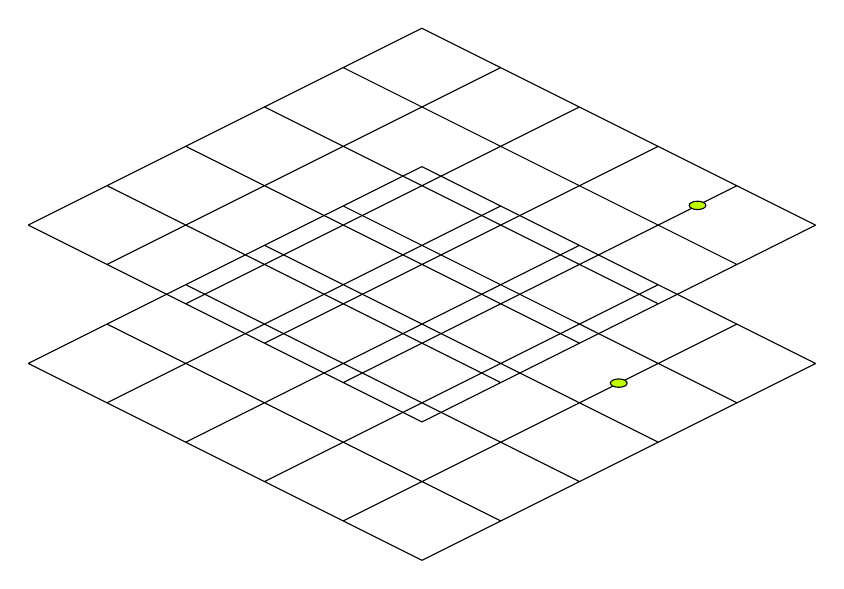
\begin{tikzpicture}
%slanting: production of a set of n 'laminae' to be piled up. N=number of grids.
    \begin{scope}[yshift=0,every node/.append style={yslant=0.5,xslant=-1},yslant=0.5,xslant=-1]
        \draw[step=10mm, black] (0,0) grid (5,5); %defining grids
        \draw [fill=lime](3.50,1.0) circle (\R);
        %Idem as above, for the n-th grid:
    \end{scope}
    \begin{scope}[yshift=50,every node/.append style={yslant=0.5,xslant=-1},yslant=0.5,xslant=-1]
        \draw[step=10mm, black] (0,0) grid (5,5); %defining grids
        \draw [fill=lime](4.50,1.0) circle (\R);
        %Idem as above, for the n-th grid:
    \end{scope}
\end{tikzpicture}
\end{document}
